\begin{figure}[h!]
    \centering
    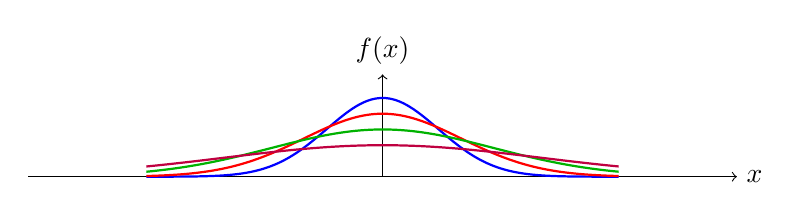
\begin{tikzpicture}
    % Draw the x and y axes
    \draw[->] (-4.5, 0) -- (4.5, 0) node[right] {$x$};
    \draw[->] (0, 0) -- (0, 1.3) node[above] {$f(x)$};

    % First normal distribution (narrowest)
    \draw[thick, blue, smooth, domain=-3:3, samples=100] 
        plot ({\x}, {exp(-\x*\x)}) node[pos=0.50, right] {};

    % Second normal distribution (wider)
    \draw[thick, red, smooth, domain=-3:3, samples=100] 
        plot ({\x}, {0.8*exp(-0.5*\x*\x)}) node[pos=0.95, right] {};

    % Third normal distribution (even wider)
    \draw[thick, green!70!black, smooth, domain=-3:3, samples=100] 
        plot ({\x}, {0.6*exp(-0.25*\x*\x)}) node[pos=0.95, right] {};

    % Fourth normal distribution (widest)
    \draw[thick, purple, smooth, domain=-3:3, samples=100] 
        plot ({\x}, {0.4*exp(-0.125*\x*\x)}) node[pos=0.95, right] {} ;
\end{tikzpicture}
\end{figure}
